\newpage
\subsection{UC4 - Modifica visualizzazione}
\label{sub:uc4}

%TODO: Add correct image
\begin{figure}[h]
    \centering
    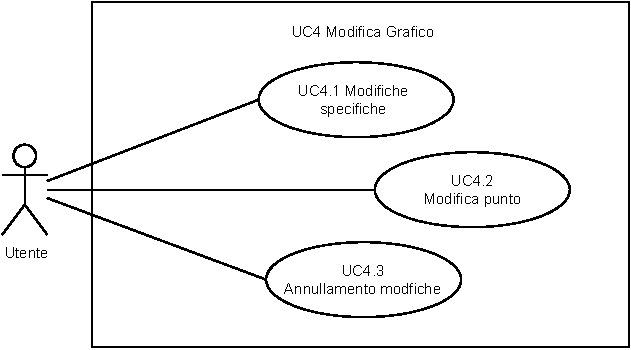
\includegraphics[width=0.8\textwidth]{componenti/casi-duso/diagrammi/UC4.pdf}
    \caption{Diagramma rappresentante UC4}
    \label{fig:UC4}
\end{figure}


\begin{itemize}
    \item \textbf{Descrizione}: L’utente modifica il grafico attuale del quale viene fornita la visualizzazione aggiornata.
	
    \item \textbf{Attore primario}: Utente.
    
    \item \textbf{Precondizione}:   È stato costruito correttamente un grafico (UC2 \refSec{sub:uc2})

    \item \textbf{Postcondizione}:  Viene visualizzato il grafico modificato con i nuovi parametri.

	\item \textbf{Scenario principale}:
		\begin{enumerate}
            \item L'utente modifica i parametri di visualizzazione, interagendo con gli strumenti resi disponbili dal grafico che sta visualizzando,
                    dal menu di modifica.
            \item La visualizzazione del grafico viene aggiornata in accordo con i parametri modificati.
        \end{enumerate}

    \item \textbf{Scenario alternativo}:
        \begin{enumerate}
            \item L'utente seleziona la voce "Annulla" dal menù di modifica.
            \item Le modifiche vengono scartate e viene ripristinata la visualizzazione del grafico precedente.  (UC4.8)
        \end{enumerate}
    
\end{itemize}

\newpage
\subsubsection{UC4.1 Modifica grafico}
\label{ssub:uc4.1}

\begin{itemize}
    \item \textbf{Descrizione}: L’utente effettua modifica specifiche al tipo di grafico precedentemente costruito e visualizzato, 
                                su parametri quindi validi solo per tale visualizzazone, e ne vede le modifiche.
	
    \item \textbf{Attore primario}: Utente.
    
    \item \textbf{Precondizione}:   È stato costruito correttamente un grafico. (UC2 \refSec{sub:uc2})

    \item \textbf{Postcondizione}:  Viene aggiornato il grafico costruito e visualizzato con i nuovi parametri.

    \item \textbf{Generalizzazioni}:
        \begin{itemize}
            \item Modifica Scatterplot Matrix (UC4.2 \refSec{ssub:uc4.2})
            \item Modifica a grafico con Matrice delle Distanze (UC4.3 \refSec{ssub:uc4.3})
            \begin{itemize}
                \item Modifica Force Field (UC4.4 \refSec{ssub:uc4.4})
                \item Modifica Distance Map (UC4.5 \refSec{ssub:uc4.5})
             \end{itemize}
            \item Modifica Heat Map (UC4.6 \refSec{ssub:uc4.6})
            \item Modifica Proiezione Lineare Multi Asse (UC4.7 \refSec{ssub:uc4.7})
        \end{itemize}
\end{itemize}

\subsubsection{UC4.2 Modifica Scatterplot Matrix}
\label{ssub:uc4.2}

\begin{figure}[h]
    \centering
    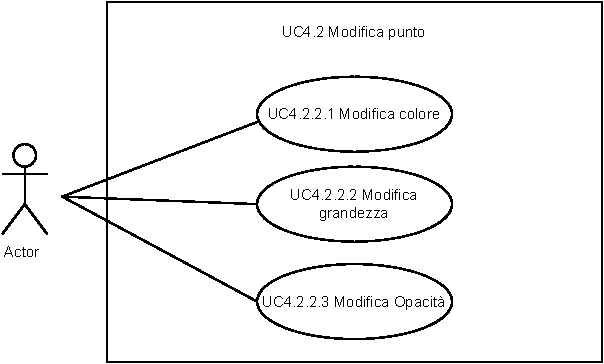
\includegraphics[width=0.6\textwidth]{componenti/casi-duso/diagrammi/UC4_2.pdf}
    \caption{Diagramma rappresentante UC4.2}
    \label{fig:UC4.2}
\end{figure}


\begin{itemize}
    \item \textbf{Descrizione}: L’utente modifica la visualizzazione dello Scatterplot Matrix
                                costruito dal dataset corrente.
	
    \item \textbf{Attore primario}: Utente.
    
    \item \textbf{Precondizione}:   La visualizzazione costruita dal dataset corrente è uno Scatterplot Matrix.

    \item \textbf{Postcondizione}:  Viene aggiornato il grafico costruito e visualizzato con i nuovi parametri.

	\item \textbf{Scenario principale}:
		\begin{enumerate}
            \item L'utente apporta le modifiche desiderate tra quelle offerte dallo Scatterplot Matrix.
        \end{enumerate}
\end{itemize}


\subsubsection{UC4.2.1 Modifica dimensioni della matrice}
\label{ssub:uc4.2.1}
\begin{itemize}
    \item \textbf{Descrizione}:     L’utente dispone di dati con metadati assegnati e può 
                                    scegliere fino a 5 dimensioni che possono essere visualizzate nello Scatter Plot 
                                    Matrix.
	
    \item \textbf{Attore primario}: Utente.
    
    \item \textbf{Precondizione}:   La visualizzazione costruita dal dataset corrente è uno Scatterplot Matrix.
    \item \textbf{Postcondizione}:  Vengono modificate le dimensioni visualizzate nei plot dello Scatter Plot Matrix.

	\item \textbf{Scenario principale}:
        \begin{enumerate}
            \item   L'utente seleziona l'opzione di selezione delle dimensioni.
            \item   L'utente seleziona fino a cinque dimensioni. 
           
            \item   Ad ogni selezione l'utente
                    sceglie una delle dimensioni attuali del grafico e la scarta.
           
            \item   La visualizzazione sostituisce le dimensioni scartate con le nuove selezionate.
        \end{enumerate}
\end{itemize}

\subsubsection{UC4.2.2 Modifica dimensione rappresentata mediante tinta}
\label{ssub:uc4.2.2}
\begin{itemize}
    
    \item \textbf{Descrizione}:     L'utente assegna ad una dimensione un insieme di tinte per poterla rappresentare 
                                    graficamente;
    
    \item \textbf{Attore primario}: Utente;
    \item \textbf{Precondizione}:   La visualizzazione correntemente costruita dal dataset è uno Scatter Plot Matrix;
    \item \textbf{Postcondizione}:  Viene aggiunta una dimensione rappresentata mediante tinta;
    \item \textbf{Scenario principale}:
    \begin{enumerate}
        
        \item   Interagendo con l'apposito pulsante, l'utente seleziona la dimensione che desidera rappresentare 
                mediante tinta, sostituendo così quella precedente;

        \item   L'utente seleziona tra gli intervalli di tinte suggeriti quello con cui i diversi elementi della 
                dimensione scelta saranno visualizzati;
        
        \item   La visualizzazione viene aggiornata in accordo con le modifiche effettuate.
    \end{enumerate}
\end{itemize}

\subsubsection{UC4.2.3 Modifica dimensione rappresentata mediante brillanza}
\label{ssub:uc4.2.3}
\begin{itemize}

    \item \textbf{Descrizione}:     L'utente assegna ad una dimensione la rappresentazione mediante brillanza;
    \item \textbf{Attore primario}: Utente;
    \item \textbf{Precondizione}:   La visualizzazione correntemente costruita dal dataset è uno Scatter Plot Matrix;
    \item \textbf{Postcondizione}:  Viene modificata la dimensione rappresentata mediante brillanza;
    \item \textbf{Scenario principale}:
    \begin{enumerate}
        \item   Interagendo con l'apposito pulsante, l'utente seleziona la dimensione che desidera rappresentare 
                mediante brillanza, sostituendo così quella precedente;

        \item   La visualizzazione viene aggiornata in accordo con la modifica effettuata.
    \end{enumerate}
\end{itemize}

\subsubsection{UC4.2.4 Selezione punto}
\label{ssub:uc4.2.4}
\begin{itemize}
    \item \textbf{Descrizione}: L'utente seleziona un punto in uno Scatterplot della matrice per vedere come 
                                esso viene rappresentato negli altri grafici a dispersione della visualizzazione corrente.
	
    \item \textbf{Attore primario}: Utente.
    
    \item \textbf{Precondizione}:   La visualizzazione costruita dal dataset corrente è uno Scatterplot Matrix.
    \item \textbf{Postcondizione}:  Le proiezioni del punto selezionato, se appartiene al dataset importato, 
                                    venogno evidenziate in tutti i grafici della visualizzazione.

	\item \textbf{Scenario principale}:
        \begin{enumerate}
            \item L'utente seleziona un punto contente dati di uno Scatterplot della matrice.
            \item La proiezione del punto viene evidenziata in tutti gli Scatterplot della visualizzazione.
        \end{enumerate}

    \item \textbf{Scenario alternativo}:
        \begin{enumerate}
            \item L'utente seleziona un punto che non rappresenta nessun dato del dataset.
            \item Non viene evidenziato alcun punto della matrice.
        \end{enumerate}

\end{itemize}


\subsubsection{UC4.2.5 Selezione insieme di punti}
\label{ssub:uc4.2.5}
\begin{itemize}
    \item \textbf{Descrizione}: L'utente seleziona un insieme di punti in uno Scatterplot della matrice per vedere come 
                                essi vengono rappresentati negli altri Scatterplot della matrice.
	
    \item \textbf{Attore primario}: Utente.
    
    \item \textbf{Precondizione}:   La visualizzazione costruita dal dataset corrente è uno Scatterplot Matrix.
    \item \textbf{Postcondizione}:  Le proiezioni degli insiemi di punti selezionati, se appartentente al dataset importato, 
                                    vengono evidenziate in tutti i grafici della visualizzazione.

	\item \textbf{Scenario principale}:
        \begin{enumerate}
            \item L'utente seleziona un insieme di punti di uno Scatterplot della matrice.
            \item Le proiezioni dei punti contenteni dati vengono evidenziati in tutti gli Scatterplot della visualizzazione.
        \end{enumerate}

    \item \textbf{Scenario alternativo}:
        \begin{enumerate}
            \item L'utente seleziona un insieme di punti vuoto.
            \item Non viene evidenziato alcun punto della matrice.
        \end{enumerate}

\end{itemize}

\newpage
\subsubsection{UC4.3 Modifica a grafico con matrice delle distanze}
\label{ssub:uc4.3}

% TODO: Insert UC4.3 image
\begin{figure}[h]
    \centering
    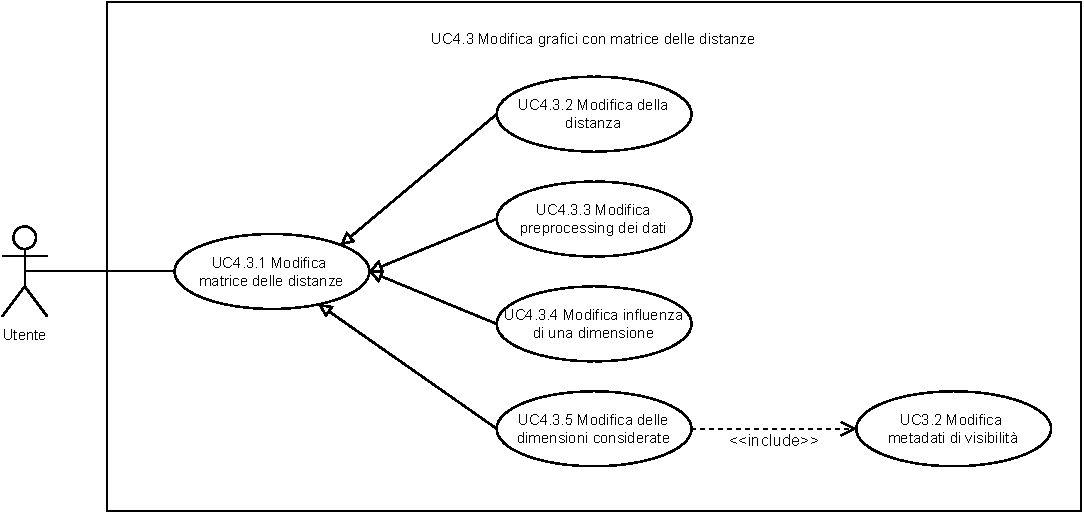
\includegraphics[width=0.8  \textwidth]{componenti/casi-duso/diagrammi/UC4_3.pdf}
    \caption{Diagramma rappresentante UC4.3}
    \label{fig:UC4.3}
\end{figure}

\begin{itemize}
    \item \textbf{Descrizione}: L’utente vuole modificare la visualizzazione di un grafico che sfrutta la matrice delle distanze
                                nella sua costruzione, Force Field o Distance Map.
    \item \textbf{Attore primario}: Utente.
    \item \textbf{Precondizione}: La visualizzazione costruita dal dataset corrente è una Force Field o una Distance Map. 
    \item \textbf{Postcondizione}: Viene aggiornato il grafico costruito e visualizzato con i nuovi parametri.
    \item \textbf{Scenario principale}:
    \begin{enumerate}
        \item   L’utente apporta le modifiche desiderate tra quelle offerte dal grafico con matrice
                delle distanze e quelle specifiche al tipo di grafico che la visualizzazione attuale rappresenta.
    \end{enumerate}
    \item \textbf{Generalizzazioni}:
    \begin{itemize}
        \item Modifica Force Field. (UC4.4)
        \item Modifica Distance Map. (UC4.5)
    \end{itemize}
    
    \item \textbf{Inclusioni}:
    \begin{itemize} 
        \item La \emph{Modifica delle dimensioni considerate} (UC4.3.5) include la modifica dei metadati di visibilità. (UC3.2)
    \end{itemize}
\end{itemize}

\subsubsection{UC4.3.1 Modifica a matrice delle distanze}
\label{ssub:uc4.3.1}
\begin{itemize}
    \item \textbf{Descrizione}:
    \item \textbf{Attore primario}:
    \item \textbf{Precondizione}:
    \item \textbf{Postcondizione}:
    \item \textbf{Scenario principale}:
    \begin{itemize}
        \item L'utente
    \end{itemize}
\end{itemize}

\subsubsection{UC4.3.2 Modifica della distanza}
\label{subsec:uc4.3.2}
\begin{itemize}
    \item \textbf{Descrizione}: L’utente decide di cambiare l’algoritmo usato per il calcolo delle distanze.

	
    \item \textbf{Attore primario}: Utente.
    
    \item \textbf{Precondizione}:   La visualizzazione costruita dal dataset corrente è un Force Field.
    \item \textbf{Postcondizione}:  Viene modificata la distanza tra i nodi del grafo nella visualizzazione.

	\item \textbf{Scenario principale}:
        \begin{enumerate}
            \item L'utente seleziona il menu delle distanze e seleziona uno degli algoritmi presentati nel menù.
            \item La visualizzazione modifica la distanza tra i nodi secondo l'algoritmo scelto.
        \end{enumerate}
\end{itemize}

\subsubsection{UC4.3.3 Modifica preprocessing dei dati}
\label{ssub:uc4.3.3}
\begin{itemize}
    \item \textbf{Descrizione}:
    \item \textbf{Attore primario}:
    \item \textbf{Precondizione}:
    \item \textbf{Postcondizione}:
    \item \textbf{Scenario principale}:
    \begin{itemize}
        \item L'utente
    \end{itemize}
\end{itemize}

\subsubsection{UC4.3.4 Modifica influenza di una dimensione}
\label{ssub:uc4.3.4}
\begin{itemize}
    \item \textbf{Descrizione}:
    \item \textbf{Attore primario}:
    \item \textbf{Precondizione}:
    \item \textbf{Postcondizione}:
    \item \textbf{Scenario principale}:
    \begin{itemize}
        \item L'utente
    \end{itemize}
\end{itemize}

\subsubsection{UC4.3.5 Modifica delle dimensioni considerate}
\label{ssub:uc4.3.5}
\begin{itemize}
    \item \textbf{Descrizione}:
    \item \textbf{Attore primario}:
    \item \textbf{Precondizione}:
    \item \textbf{Postcondizione}:
    \item \textbf{Scenario principale}:
    \begin{itemize}
        \item L'utente
    \end{itemize}
\end{itemize}

\newpage
\subsubsection{UC4.4 Modifica Force Field}
\label{ssub:uc4.4}
% TODO: Create image for force field graph.
\begin{figure}[h]
    \centering
    % 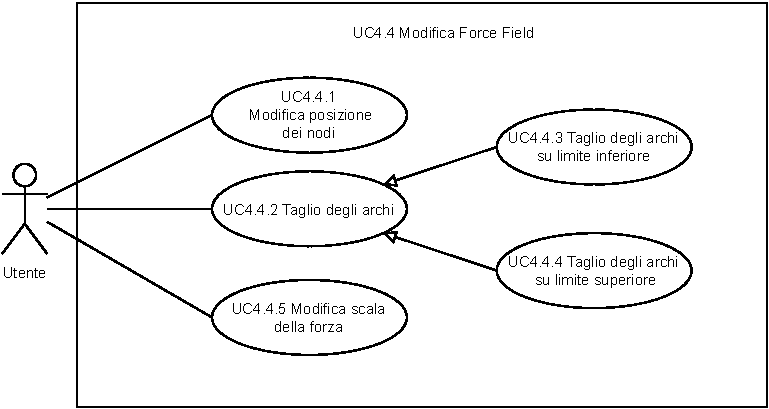
\includegraphics[width=0.6  \textwidth]{componenti/casi-duso/diagrammi/UC4_4.pdf}
    \caption{Diagramma rappresentante UC4.4}
    \label{fig:UC4.4}
\end{figure}


\begin{itemize}
    \item \textbf{Descrizione}: L’utente vuole modificare la visualizzazione del grafo Force Field
                                costruito dal dataset corrente.
	
    \item \textbf{Attore primario}: Utente.
    
    \item \textbf{Precondizione}:   La visualizzazione costruita dal dataset corrente è un Force Field.

    \item \textbf{Postcondizione}:  Viene aggiornato il grafico costruito e visualizzato con i nuovi parametri.

	\item \textbf{Scenario principale}:
		\begin{enumerate}
            \item L'utente apporta le modifiche desiderate tra quelle offerte dal Force Field.
        \end{enumerate}
\end{itemize}

\subsubsection{UC4.4.1 Modifica posizione dei nodi}
\label{ssub:uc4.4.1}
\begin{itemize}
    \item \textbf{Descrizione}: L’utente vuole esplorare meglio i dati e decide di 
                                modificare la posizione dei nodi del grafo, trascinandoli con il 
                                cursore nell'area definita dal grafico.
	
    \item \textbf{Attore primario}: Utente.
    
    \item \textbf{Precondizione}:   La visualizzazione costruita dal dataset corrente è un Force Field.
    \item \textbf{Postcondizione}:  Viene modificata la posizione dei nodi del grafo nella visualizzazione.

	\item \textbf{Scenario principale}:
        \begin{enumerate}
            \item L'utente tiene premuto il tasto di selezione e trascina il cursore sponstando il nodo nello spazio della visualizzazione.
            \item La visualizzazione muove i punti del grafo mantentendo le connessioni tra i nodi.
        \end{enumerate}
\end{itemize}

\subsubsection{UC4.4.2 Taglio degli archi}
\label{ssub:uc4.4.2}
\begin{itemize}
    \item \textbf{Descrizione}:     L'utente imposta un valore di soglia sulla distanza, gli archi corrispondenti ad una distanza che non rispetta la soglia vengono rimossi;
    \item \textbf{Attore primario}: Utente;
    \item \textbf{Precondizione}:   La visualizzazione correntemente costruita dal dataset é un Force Field;
    \item \textbf{Postcondizione}:  Viene aggiornata la visualizzazione, rimuovendo gli archi in base al valore di soglia impostato;
    \item \textbf{Scenario principale}:
    \begin{itemize}
        \item L'utente inserisce nell'apposito campo il valore di soglia;
        \item Gli archi le cui coordinate nella matrice delle distanze non rispettano il valore di soglia vengono rimossi;
        \item La visualizzazione viene aggiornata rimuovendo gli archi secondo il valore di soglia stabilito.
    \end{itemize}
\end{itemize}

\subsubsection{UC4.4.3 Taglio degli archi su limite inferiore}
\label{ssub:uc4.4.3}
\begin{itemize}
    \item \textbf{Descrizione}:     L'utente imposta un valore di soglia minimo sulla distanza, gli archi corrispondenti ad una distanza inferiore vengono rimossi;
    \item \textbf{Attore primario}: Utente;
    \item \textbf{Precondizione}:   La visualizzazione correntemente costruita dal dataset é un Force Field;
    \item \textbf{Postcondizione}:  Viene aggiornata la visualizzazione, rimuovendo gli archi associati ad una distanza inferiore al valora di soglia minimo;
    \item \textbf{Scenario principale}:
    \begin{itemize}
        \item L'utente inserisce nell'apposito campo il valore di soglia minimo;
        \item Gli archi le cui coordinate nella matrice delle distanze corrispondono ad una distanza inferiore al valore di soglia minimo vengono rimossi;
        \item La visualizzazione viene aggiornata rimuovendo gli archi con una distanza associata inferiore al valore di soglia minimo.
    \end{itemize}
\end{itemize}

\subsubsection{UC4.4.4 Taglio degli archi su limite superiore}
\label{ssub:uc4.4.4}
\begin{itemize}
    \item \textbf{Descrizione}:     L'utente imposta un valore di soglia massimo sulla distanza, gli archi corrispondenti ad una distanza superiore vengono rimossi;
    \item \textbf{Attore primario}: Utente;
    \item \textbf{Precondizione}:   La visualizzazione correntemente costruita dal dataset é un Force Field;
    \item \textbf{Postcondizione}:  Viene aggiornata la visualizzazione, rimuovendo gli archi associati ad una distanza superiore al valore di soglia massimo;
    \item \textbf{Scenario principale}:
    \begin{itemize}
        \item L'utente inserisce nell'apposito campo il valore di soglia massimo;
        \item Gli archi le cui coordinate nella matrice delle distanze corrispondono ad una distanza superiore al valore di soglia massimo vengono rimossi;
        \item La visualizzazione viene aggiornata rimuovendo gli archi con una distanza associata superiore al valore di soglia massimo.
    \end{itemize}
\end{itemize}

\subsubsection{UC4.4.5 Modifica scala della forza}
\label{ssub:uc4.4.5}
\begin{itemize}
    \item \textbf{Descrizione}: Per poter visualizzare meglio i cluster di dati l’utente 
                                decide di scalare la forza di attrattiva tra i nodi.

	
    \item \textbf{Attore primario}: Utente.
    
    \item \textbf{Precondizione}:   La visualizzazione costruita dal dataset corrente è un Force Field.
    \item \textbf{Postcondizione}:  Viene modificata l'intensità della forza attrattiva tra i nodi del grafo nella visualizzazione.

	\item \textbf{Scenario principale}:
        \begin{enumerate}
            \item L'utente seleziona la barra intensità e trascinando il cursore sulla barra varia l’intensità.
            \item La visualizzazione modifica l'intensità della forza secondo il valore selezionato nel grafo.
        \end{enumerate}
\end{itemize}

\newpage
\subsubsection{UC4.5 Modifica Distance Map}
\label{ssub:uc4.5}
% TODO: Insert image for Distance Map
\begin{figure}[h]
    \centering
    % 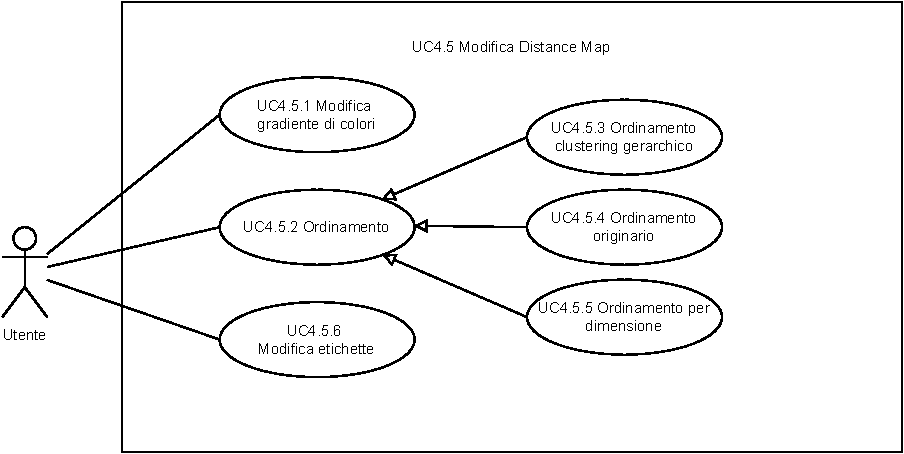
\includegraphics[width=0.8\textwidth]{componenti/casi-duso/diagrammi/UC4_5.pdf}
    \caption{Diagramma rappresentante UC4.5}
    \label{fig:UC4.2}
\end{figure}

\begin{itemize}
    \item \textbf{Descrizione}:
    \item \textbf{Attore primario}:
    \item \textbf{Precondizione}:
    \item \textbf{Postcondizione}:
    \item \textbf{Scenario principale}:
    \begin{itemize}
        \item L'utente
    \end{itemize}
\end{itemize}

\subsubsection{UC4.5.1 Modifica della scala di colori}
\label{ssub:uc4.5.1}
\begin{itemize}
    \item \textbf{Descrizione}:
    \item \textbf{Attore primario}:
    \item \textbf{Precondizione}:
    \item \textbf{Postcondizione}:
    \item \textbf{Scenario principale}:
    \begin{itemize}
        \item L'utente
    \end{itemize}
\end{itemize}

\subsubsection{UC4.5.2 Ordinamento delle righe}
\label{ssub:uc4.5.2}
\begin{itemize}
    \item \textbf{Descrizione}:
    \item \textbf{Attore primario}:
    \item \textbf{Precondizione}:
    \item \textbf{Postcondizione}:
    \item \textbf{Scenario principale}:
    \begin{itemize}
        \item L'utente
    \end{itemize}
\end{itemize}

\subsubsection{UC4.5.3 Ordinamento delle colonne}
\label{ssub:uc4.5.3}
\begin{itemize}
    \item \textbf{Descrizione}:
    \item \textbf{Attore primario}:
    \item \textbf{Precondizione}:
    \item \textbf{Postcondizione}:
    \item \textbf{Scenario principale}:
    \begin{itemize}
        \item L'utente
    \end{itemize}
\end{itemize}

\subsubsection{UC4.5.4 Visualizzazione etichette di riga}
\label{ssub:uc4.5.4}
\begin{itemize}
    \item \textbf{Descrizione}:
    \item \textbf{Attore primario}:
    \item \textbf{Precondizione}:
    \item \textbf{Postcondizione}:
    \item \textbf{Scenario principale}:
    \begin{itemize}
        \item L'utente
    \end{itemize}
\end{itemize}

\subsubsection{UC4.5.5 visualizzazione etichette di colonna}
\label{ssub:uc4.5.5}
\begin{itemize}
    \item \textbf{Descrizione}:
    \item \textbf{Attore primario}:
    \item \textbf{Precondizione}:
    \item \textbf{Postcondizione}:
    \item \textbf{Scenario principale}:
    \begin{itemize}
        \item L'utente
    \end{itemize}
\end{itemize}

\subsubsection{UC4.5.6 Modifica etichette di riga}
\label{ssub:uc4.5.6}
\begin{itemize}
    \item \textbf{Descrizione}:
    \item \textbf{Attore primario}:
    \item \textbf{Precondizione}:
    \item \textbf{Postcondizione}:
    \item \textbf{Scenario principale}:
    \begin{itemize}
        \item L'utente
    \end{itemize}
\end{itemize}

\subsubsection{UC4.5.7 Modifica etichette di colonna}
\label{ssub:uc4.5.7}
\begin{itemize}
    \item \textbf{Descrizione}:
    \item \textbf{Attore primario}:
    \item \textbf{Precondizione}:
    \item \textbf{Postcondizione}:
    \item \textbf{Scenario principale}:
    \begin{itemize}
        \item L'utente
    \end{itemize}
\end{itemize}

\newpage
\subsubsection{UC4.6 Modifica Proiezione Lineare Multi Asse}
\label{ssub:uc4.6}
% TODO: Create image for PLMA
\begin{figure}[h]
    \centering
    % 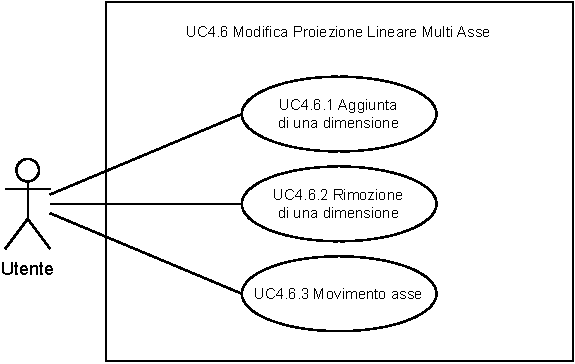
\includegraphics[width=0.8\textwidth]{componenti/casi-duso/diagrammi/UC4_6.pdf}
    \caption{Diagramma rappresentante UC4.6}
    \label{fig:UC4.6}
\end{figure}

\begin{itemize}
    \item \textbf{Descrizione}: L’utente vuole modificare la visualizzazione della Proiezione Lineare Multi Asse
                                costruita dal dataset corrente.
	
    \item \textbf{Attore primario}: Utente.
    
    \item \textbf{Precondizione}:   La visualizzazione costruita dal dataset corrente è un grafico di tipo Proiezione Lineare Multi Asse.
    \item \textbf{Postcondizione}:  Viene aggiornato il grafico costruito e visualizzato con i nuovi parametri.

	\item \textbf{Scenario principale}:
		\begin{enumerate}
            \item L'utente apporta le modifiche desiderate tra quelle offerte dalla Proiezione Lineare Multi Asse.
        \end{enumerate}
\end{itemize}

\subsubsection{UC4.6.1 Aggiunta dimensione}
\label{ssub:uc4.6.1}
\begin{itemize}
    \item \textbf{Descrizione}: L’utente decide di visualizzare maggiori informazioni
                                aggiungendo una dimensione al grafico.

    \item \textbf{Attore primario}: Utente.
    
    \item \textbf{Precondizione}:   La visualizzazione costruita corrente è una Proiezione Lineare Multi Asse
                                    e rappresenta al più una dimensione in meno al numero di dimensioni del dataset.
    \item \textbf{Postcondizione}:  La visualizzazione della PLA aggiunge una dimenisone.

	\item \textbf{Scenario principale}:
        \begin{enumerate}
            \item L'utente seleziona la voce "Dimensioni" e seleziona una dimensione da aggiungere alla proiezione.
            \item La visualizzazione aggiugne la dimensione selezionata e riposiziona i punti.
           
        \end{enumerate}
\end{itemize}

\subsubsection{UC4.6.2 Rimozione dimensione}
\label{ssub:uc4.6.2}
\begin{itemize}
    \item \textbf{Descrizione}: L’utente decide di rimuovere una dimensione dalla Proiezione Lineare Multi Asse
                                a patto che essa non sia monodimensionale.

    \item \textbf{Attore primario}: Utente.
    
    \item \textbf{Precondizione}:   La visualizzazione costruita dal dataset corrente è una Proiezione Lineare Multi Asse
                                    e rappresenta almeno due dimensioni.
    \item \textbf{Postcondizione}:  La visualizzazione della PLA rimuove una dimenisone.

	\item \textbf{Scenario principale}:
        \begin{enumerate}
            \item L'utente seleziona la voce "Dimensioni" e seleziona una dimensione da rimuovere dalla proiezione.
            \item La visualizzazione rimuove la dimensione selezionata e riposiziona i punti.
           
        \end{enumerate}
\end{itemize}

\subsubsection{UC4.6.3 Rotazione asse}
\label{ssub:uc4.6.3}
\begin{itemize}
    \item \textbf{Descrizione}:
    \item \textbf{Attore primario}:
    \item \textbf{Precondizione}:
    \item \textbf{Postcondizione}:
    \item \textbf{Scenario principale}:
    \begin{enumerate}
        \item L'utente
    \end{enumerate}
\end{itemize}

\newpage
\subsubsection{UC4.7 Modifica Heat Map}
\label{ssub:uc4.7}
% TODO: Create image for force field graph.
\begin{figure}[h]
    \centering
    % 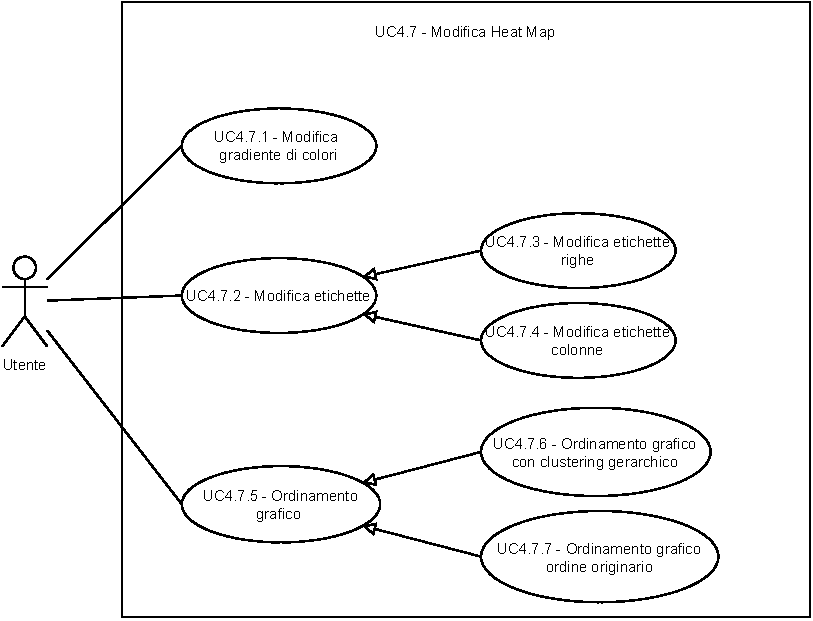
\includegraphics[width=0.6\textwidth]{componenti/casi-duso/diagrammi/UC4_7.pdf}
    \caption{Diagramma rappresentante UC4.7}
    \label{fig:UC4.7}
\end{figure}


\begin{itemize}
    \item \textbf{Descrizione}: L’utente vuole modificare la visualizzazione della Heat Map
                                costruita dal dataset corrente.
	
    \item \textbf{Attore primario}: Utente.
    
    \item \textbf{Precondizione}:   La visualizzazione costruita dal dataset corrente è un grafico di tipo Heat Map.

    \item \textbf{Postcondizione}:  Viene aggiornato il grafico costruito e visualizzato con i nuovi parametri.

	\item \textbf{Scenario principale}:
		\begin{enumerate}
            \item L'utente apporta le modifiche desiderate tra quelle offerte dalla Heat Map.
        \end{enumerate}
\end{itemize}

\subsubsection{UC4.7.1 Modifica scala dei colori}
\label{ssub:uc4.7.1}
\begin{itemize}
    \item \textbf{Descrizione}: L’utente vuole esplorare meglio i dati e decide di 
                                modificare la scala dei colori applicata alla Heat Map scegliendo una 
                                tra quelle proposte.
	
    \item \textbf{Attore primario}: Utente.
    
    \item \textbf{Precondizione}:   La visualizzazione costruita dal dataset corrente è una Heat Map.
    \item \textbf{Postcondizione}:  Viene modificata la scala dei colori del grafico nella visualizzazione.

	\item \textbf{Scenario principale}:
        \begin{enumerate}
            \item L'utente seleziona la voce "Scala dei colori" e seleziona una delle opzioni disponibili.
            \item La visualizzazione cambia la scala dei colori adottata dalla Heat Map.
        \end{enumerate}
\end{itemize}

\subsubsection{UC4.7.2 Ordinamento delle righe}
\label{ssub:uc4.7.2}
\begin{itemize}
    \item \textbf{Descrizione}: L’utente per esplorare meglio i dati decide di ordinare le righe della Heat Map
                                seguendo l'algortimo di clustering gerarchico il quale aggiunge un dendogramma alla visualizzazione corrente.
	
    \item \textbf{Attore primario}: Utente.
    
    \item \textbf{Precondizione}:   La visualizzazione costruita dal dataset corrente è una Heat Map.
    \item \textbf{Postcondizione}:  Le righe della Heat Map vengono visualizzati secondo l'ordine imposto dall'algoritmo di ordinamento.

	\item \textbf{Scenario principale}:
        \begin{enumerate}
            \item   L'utente seleziona la casella di ordinamento delle righe.
            \item   La visualizzazione aggiorna l'ordinamento delle righe della Heat Map e viene aggiunto 
                    il dendogramma relativo alle righe.
        \end{enumerate}
\end{itemize}

\subsubsection{UC4.7.3 Ordinamento delle colonne}
\label{ssub:uc4.7.3}
\begin{itemize}
    \item \textbf{Descrizione}: L’utente per esplorare meglio i dati decide di ordinare le colonne della Heat Map
                                seguendo l'algortimo di clustering gerarchico il quale aggiunge un dendogramma alla visualizzazione corrente.
	
    \item \textbf{Attore primario}: Utente.
    
    \item \textbf{Precondizione}:   La visualizzazione costruita dal dataset corrente è una Heat Map..
    \item \textbf{Postcondizione}:  Le colonne della Heat Map vengono visualizzati secondo l'ordine imposto dall'algoritmo di ordinamento.

	\item \textbf{Scenario principale}:
        \begin{enumerate}
            \item   L'utente seleziona la casella di ordinamento delle colonne.
            \item   La visualizzazione aggiorna l'ordinamento delle colonne della Heat Map 
                    e viene aggiunto il dendogramma relativo alle righe.
        \end{enumerate}
\end{itemize}


\subsubsection{UC4.7.4 Visualizzazione etichette di riga}
\label{ssub:uc4.7.4}
\begin{itemize}
    \item \textbf{Descrizione}: L’utente decide se visualizzare le etichette relative alle righe della Heat Map.

    \item \textbf{Attore primario}: Utente.
    
    \item \textbf{Precondizione}:   La visualizzazione costruita dal dataset corrente è una Heat Map.
    \item \textbf{Postcondizione}:  La visualizzazione della Heat Map mostra le etichette delle righe se così scelto dall'utente.

	\item \textbf{Scenario principale}:
        \begin{enumerate}
            \item   L'utente seleziona se visualizzare le etichette per le righe della Heat Map.
            \item   La visualizzazione aggiorna la visibilità delle etichette delle righe in base alla selezione dell'utente.
                    
        \end{enumerate}
\end{itemize}



\subsubsection{UC4.7.5 Visualizzazione etichette di colonna}
\label{ssub:uc4.7.5}
\begin{itemize}
    \item \textbf{Descrizione}: L’utente decide se visualizzare le etichette relative alle colonne della Heat Map.

    \item \textbf{Attore primario}: Utente.
    
    \item \textbf{Precondizione}:   La visualizzazione costruita dal dataset corrente è una Heat Map.
    \item \textbf{Postcondizione}:  La visualizzazione della Heat Map mostra le etichette delle colonne se così scelto dall'utente.

	\item \textbf{Scenario principale}:
        \begin{enumerate}
            \item   L'utente seleziona se visualizzare le etichette per le colonne della Heat Map.
            \item   La visualizzazione aggiorna la visibilità delle etichette delle colonne in base alla selezione dell'utente.
                    
        \end{enumerate}
\end{itemize}

\subsubsection{UC4.7.6 Modifica etichette di riga}
\label{ssub:uc4.7.6}
\begin{itemize}
    \item \textbf{Descrizione}: L’utente decide di modificare una o più etichette associate alla Heat Map.

    \item \textbf{Attore primario}: Utente.
    
    \item \textbf{Precondizione}:   La visualizzazione costruita dal dataset corrente è una Heat Map.
    \item \textbf{Postcondizione}:  Le etichette della Heat Map vengono aggiornate se modificate.
	\item \textbf{Scenario principale}:
        \begin{enumerate}
            \item   L'utente seleziona le etichette da modificare e le modifica.
            \item   La visualizzazione aggiorna le etichette della Heat Map. %todo: rimuovo? 
        \end{enumerate}
\end{itemize}

\subsubsection{UC4.7.7 Aggiunta dimensione}
\label{ssub:4.7.7}
\begin{itemize}
    \item \textbf{Descrizione}:
    \item \textbf{Attore primario}:
    \item \textbf{Precondizione}:
    \item \textbf{Postcondizione}:
    \item \textbf{Scenario principale}:
    \begin{enumerate}
        \item L'utente
    \end{enumerate}
\end{itemize}

\subsubsection{UC4.7.8 Rimozione dimensione}
\label{ssub:4.7.8}
\begin{itemize}
    \item \textbf{Descrizione}:
    \item \textbf{Attore primario}:
    \item \textbf{Precondizione}:
    \item \textbf{Postcondizione}:
    \item \textbf{Scenario principale}:
    \begin{enumerate}
        \item L'utente
    \end{enumerate}
\end{itemize}

\subsection{UC4.8 Annullamento delle modifiche}
\label{ssub:uc4.8}
\begin{itemize}
    \item \textbf{Descrizione}: L'utente decide di scartare le modifiche fatte nella corrente selezione di modifica.

    \item \textbf{Attore primario}: Utente.
    
    \item \textbf{Precondizione}:   L'utente ha selezionato la voce di Modifica Grafico dal menu.
    \item \textbf{Postcondizione}:  Viene ripristinato il grafo ai parametri precedenti della selezione e visualizzato.

	\item \textbf{Scenario principale}:
        \begin{enumerate}

            \item L'utente seleziona il pulsante "Annulla modifiche".
            \item HDviz ripristina i parametri del grafo ai valori precedenti alla selezione del menu di modifica.
        
        \end{enumerate}
\end{itemize}



